% ==========================================
% BAB V IMPLEMENTASI
% ==========================================
\cleardoublepage
\chapter{IMPLEMENTASI PURWARUPA SISTEM}
\label{chap:implementasi}

Bab ini menguraikan realisasi dari rancangan sistem yang telah dibahas pada bab sebelumnya menjadi suatu aplikasi berbasis web yang diberi nama Equilibria yang berarti keseimbangan. Penjelasan dalam bab ini akan dimulai dari spesifikasi lingkungan pengembangan, persiapan instrumen materi pembelajaran, hingga detail implementasi teknis sisi peladen (\textit{backend}) dan antarmuka (\textit{frontend}).

\section{Arsitektur dan Lingkungan Pengembangan Sistem}
\label{sec:development_environment}

Implementasi sistem Equilibria membutuhkan lingkungan pengembangan dan pemilihan teknologi yang dapat mendukung proses komputasi asinkron dan isolasi eksekusi kueri. Isolasi kueri diperlukan untuk menjamin keamanan data operasional sistem saat mengevaluasi eksekusi kueri SQL dari pemelajar. Sistem ini diimplementasikan menggunakan arsitektur \textit{client-server} dengan rincian perangkat lunak sebagai berikut:

\begin{enumerate}
    \item \textbf{\textit{Backend:}} Menggunakan FastAPI (Python 3.12) sebagai \textit{framework} web asinkron utama. Pemilihan Python didasarkan pada dukungan ekosistem pustaka komputasi ilmiah (seperti NumPy) yang matang, yang krusial untuk menangani perhitungan matematis algoritma \textit{Elo rating} dan logika statistik \textit{Re-ranking} secara efisien. Kerangka kerja FastAPI dipilih untuk memastikan performa tinggi dalam melayani permintaan data secara asinkron. Interaksi basis data dikelola melalui SQLAlchemy 2.0 sebagai \textit{Object-Relational Mapper} (ORM). Fokus utama pengembangan sistem dititikberatkan pada \textit{backend} karena inti dari sistem ini terletak pada implementasi algoritma \textit{Elo rating} dan algoritma \textit{re-ranking} yang diimplementasikan di sisi \textit{backend}.
    \item \textbf{\textit{Frontend:}} Dibangun menggunakan React.js >= 19.x dengan \textit{build tool} Vite 5.x. Pengembangan antarmuka menggunakan React.js didasarkan pada arsitektur berbasis komponen dan mekanisme \textit{Virtual DOM} yang memungkinkan pembaruan tampilan secara responsif. Hal ini penting untuk menyajikan visualisasi perkembangan kompetensi secara hampir \textit{real-time} dan interaksi yang dinamis tanpa membebani peramban pengguna. Editor kode SQL menggunakan integrasi pustaka CodeMirror 6. Sebagian besar implementasi kode untuk \textit{frontend} dibantu dengan penggunaan kakas kecerdasan buatan bernama \textit{Kimi} karena tujuan pengembangan \textit{frontend} pada prototipe ini lebih ke arah menunjang kemudahan pengujian.
    \item \textbf{Basis Data:} Menggunakan PostgreSQL 15.x. Mengingat sifat data skor Elo yang transaksional dan bergantung pada integritas riwayat sebelumnya (\textit{stateful}), sistem menggunakan PostgreSQL yang menawarkan kepatuhan ACID ketat serta fitur MVCC (\textit{Multi-Version Concurrency Control}) untuk menangani konkurensi data secara andal saat banyak pemelajar berinteraksi dengan sistem secara bersamaan. Basis data dipisahkan secara logis menjadi dua skema: skema \texttt{public} untuk data operasional sistem dan skema \texttt{sandbox} untuk lingkungan eksekusi \textit{query} SQL pemelajar. Pemisahan ini bertujuan untuk mengisolasi eksekusi kueri pemelajar agar tidak mencemari skema operasional sistem. Pengaturan dan penyiapan basis data hampir keseluruhannya dilakukan manual tanpa menggunakan kakas kecerdasan buatan karena sifatnya yang lebih teknis dan melibatkan interaksi langsung dengan sistem operasi atau lingkungan eksekusi.
\end{enumerate}

Implementasi arsitektur \textit{client-server} dengan teknologi di atas cukup sederhana dan dapat dimodelkan dengan diagram pada Gambar \ref{fig:equilibria_architecture} di bawah ini.

\begin{figure}[!ht]
    \centering
    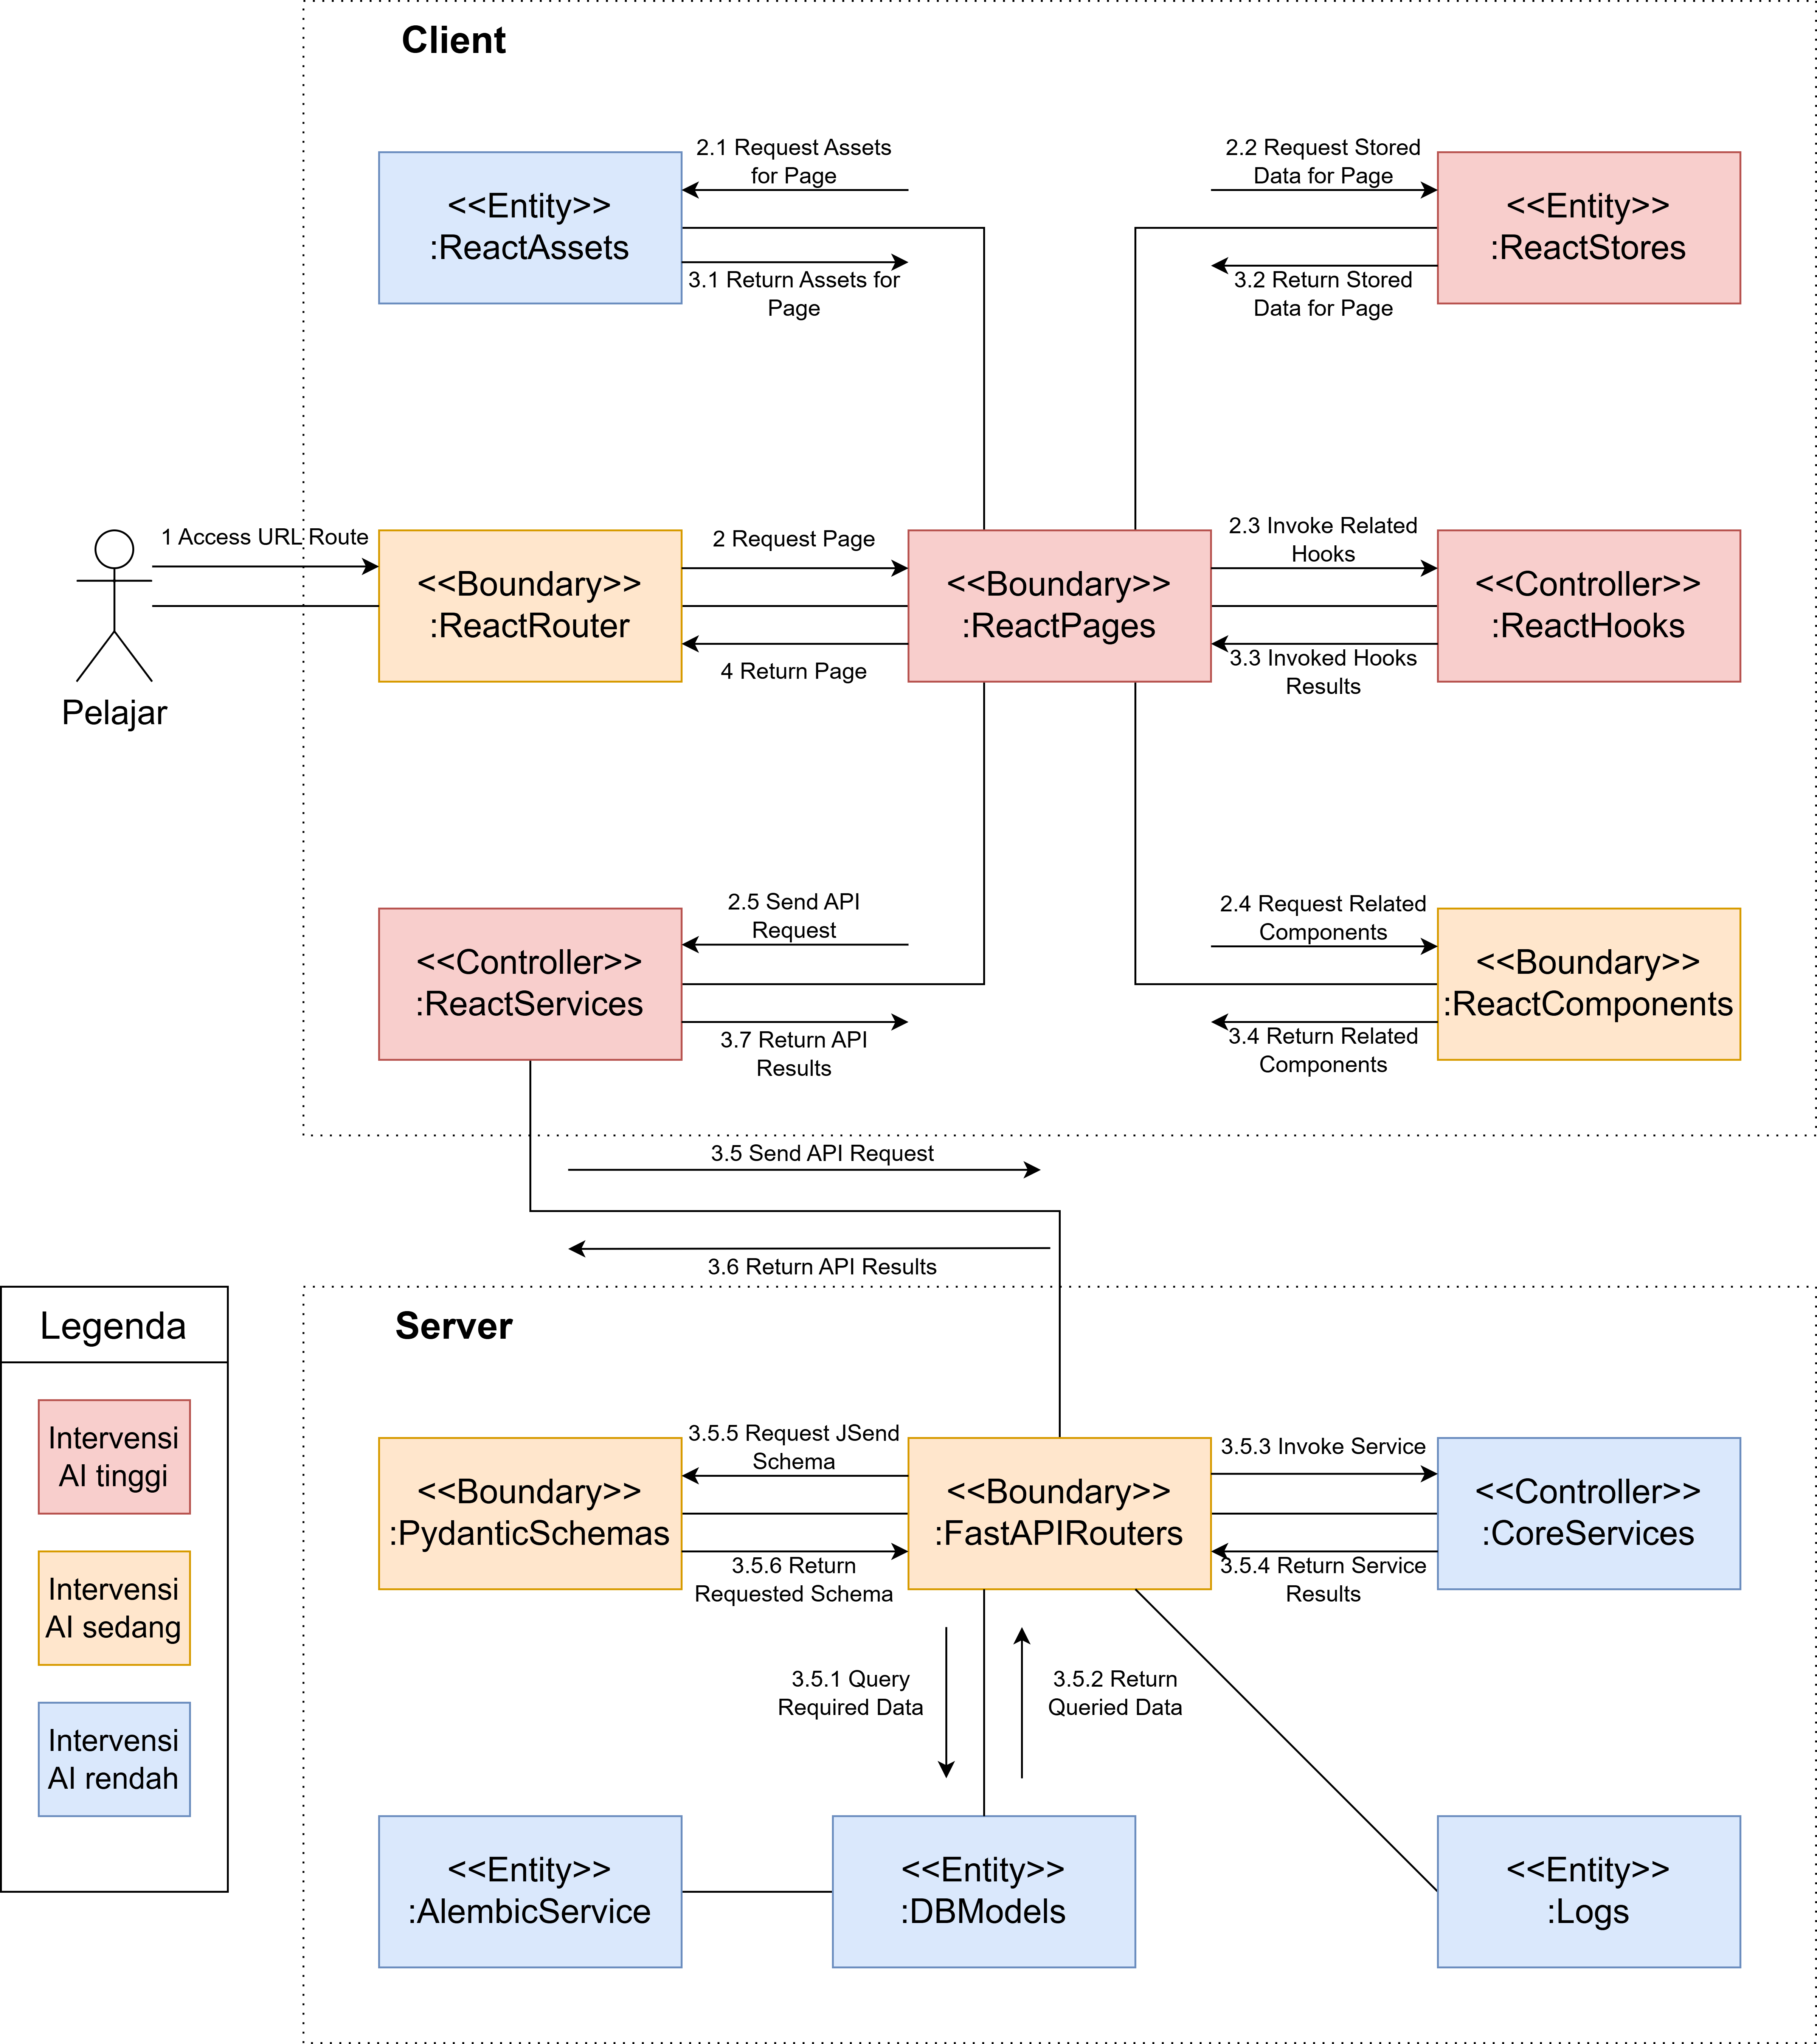
\includegraphics[width=1\textwidth]{images/equilibira_architecture.png}
    \caption{Diagram arsitektur \textit{client-server} untuk Equilibria}
    \label{fig:equilibria_architecture}
\end{figure}

Gambar \ref{fig:equilibria_architecture} menggunakan notasi \textit{communication diagram} dari UML (\textit{Unified Modeling Language}) untuk menggambarkan komponen dan interaksinya dalam sistem yang diimplementasi. Secara umum setiap komponen digambarkan dengan persegi panjang, dengan jenis komponennya diapit dua tanda kurang dari (<<) dan lebih dari (>>). Warna pada persegi panjang mengindikasikan intervensi AI dalam proses implementasinya, warna biru menunjukkan intervensi rendah, warna jingga menunjukkan intervensi sedang, dan warna merah menunjukkan intervensi tinggi. Selain penggambaran komponen, diagram tersebut juga menunjukkan alur komunikasi. Dalam rangka menyederhanakan penggambaran alur komunikasi, hanya alur komunikasi umum yang digambarkan pada diagram. Urutan alur komunikasi ditunjukkan dengan nomor urut yang ada di awal setiap pesan, tetapi perlu ditekankan bahwa untuk sub-sub langkah kedua (2.x) dan langkah ketiga (3.x) pada kenyataannya bisa terjadi secara paralel.

Jika diperhatikan pada gambar, ada dua komponen yang mungkin terlihat janggal yaitu, komponen \textit{Logs} dan komponen \textit{AlembicService}. Tidak ada pesan yang keluar atau masuk pada komponen \textit{Logs} ini karena pada saat beroperasi, pencatatan log pada umumnya terjadi beberapa kali setiap kali adanya kejadian, sehingga sulit digambarkan alur pencatatan asinkron yang berulang ini. Kasus khusus untuk komunikasi dua arah antara komponen \textit{Logs} dengan komponen \textit{FastAPI Routers} terjadi hanya ketika admin perlu membaca log yang dituliskan, maka komponen \textit{Logs} akan membalas komponen \textit{FastAPI Routers} dengan pesan "\textit{Return Logs}" atau semacamnya. Selanjutnya, untuk komponen \textit{AlembicService}, komponen ini terlibat komunikasi dengan komponen lain yaitu, \textit{DBModels} hanya ketika pengembang melakukan migrasi basis data. Dengan alasan tersebut, pada diagram komunikasi umum seperti pada Gambar \ref{fig:equilibria_architecture}, komunikasi kedua komponen ini tidak digambarkan.

\section{Persiapan Materi dan Instrumen Bank Soal}
\label{sec:persiapan_materi}

Sebelum melakukan implementasi algoritma, dilakukan penyusunan instrumen materi yang menjadi basis pembelajaran adaptif. Bagian ini merinci struktur kurikulum serta logika penetapan parameter instrumen.

\subsection{Struktur Kurikulum dan Distribusi Bank Soal}
Materi pembelajaran disusun berdasarkan kurikulum mata kuliah \textbf{IF2040 - Pemodelan Basis Data} STEI ITB tahun 2024. Materi dibagi ke dalam tiga modul sekuensial: (1) CH01 yang konten utamanya menguji konsep dasar kueri basis data (\textit{Basic Selection}), (2) CH02 yang konten utamanya menguji konsep lebih lanjut seperti penggabungan tabel dan agregasi (\textit{Aggregation}), dan (3) CH03 yang konten utamanya menguji konsep lebih lanjut mengenai kueri kompleks seperti \textit{subquery} dan \textit{Common Table Expressions} (CTEs) (\textit{Advanced Querying}).

Setiap modul dilengkapi dengan bank soal berisi \textbf{20 butir soal} dengan tingkat kesulitan yang bervariasi, sehingga total keseluruhan materi mencakup \textbf{60 butir soal}. Penentuan kuantitas ini merujuk pada temuan \textcite{Vesin2022} yang menyatakan bahwa konvergensi optimal kemahiran pemelajar dalam sistem adaptif tercapai dalam rata-rata \textbf{10 iterasi}. Dengan menyediakan 20 soal per modul, sistem menjamin variasi yang cukup untuk mencegah pemelajar menghafal jawaban (\textit{answer memorization}) serta memberikan ruang bagi algoritma untuk melakukan kalibrasi ulang terhadap tingkat kesulitan soal secara dinamis. Selain itu, penggunaan total 60 butir soal ini juga sejalan dengan penelitian \textcite{Hadi2022} yang membuktikan bahwa bank soal dengan ukuran tersebut sudah memadai dan andal untuk implementasi sistem asesmen adaptif skala kelas.

\subsection{Kalkulasi Ambang Batas Transisi Modul}
Sistem menerapkan batasan skor \textit{Elo rating} untuk mengontrol progres pemelajar antarmodul dengan ambang batas: CH01 (0), CH02 (1300), dan CH03 (1500), basis nilai tengah 1300 diadaptasi dari \textcite{Vesin2022}. Penetapan selisih 200 poin antara CH02 dan CH03 didasarkan pada asumsi 10 iterasi sukses untuk mencapai penguasaan modul. Berdasarkan kalkulasi algoritma \textit{Elo rating} yang dimodifikasi, estimasi kenaikan skor rata-rata per soal ($\Delta\theta$) dihitung dengan asumsi pemelajar menjawab benar pada median waktu pengerjaan ($t_i = 0,5 d_i$) sebagai berikut:
\begin{enumerate}
    \item Diketahui parameter diskriminasi waktu $a_i = 10^{-6}$ dan batas waktu $d_i = 300.000$ms (keduanya diadopsi dari penelitian \textcite{Vesin2022}), maka komponen waktu $a_i(d_i - t_i) = 10^{-6}(300.000 - 150.000) = 0,15$.
    \item Nilai keberhasilan dihitung melalui Persamaan \ref{eq:rumus_W_elo} (asumsi pengerjaan benar dalam satu kali percobaan): $W = 1 \times (1 + 0,15) = 1,15$.
    \item Dengan $K=30$ dan $W_e=0,5$ (saat kemampuan setara kesulitan), maka $\Delta\theta = 30(1,15 - 0,5) = 19,5 \approx 20$.
\end{enumerate}
Dengan kenaikan $\approx 20$ poin per soal, maka 10 iterasi sukses akan menghasilkan peningkatan kemahiran sebesar 200 poin, yang menjadi dasar logis perpindahan ke modul berikutnya.

\subsection{Evaluasi Kualitas Umpan Balik Berbasis NLP}
Penilaian pada aktivitas kolaboratif (\textit{Social Elo rating}) diimplementasikan melalui modul evaluasi teks otomatis yang menguantifikasi kualitas umpan balik dari pemelajar sebagai \textit{reviewer}. Sistem menggunakan model \textit{embedding} bahasa alami untuk menilai kedalaman semantik dan relevansi komentar pemelajar:

\begin{enumerate}
    \item \textbf{Model Bahasa Multilingual MiniLM:} Sistem memanfaatkan model \linebreak \textbf{\textit{paraphrase-multilingual-MiniLM-L12-v2}} untuk merepresentasikan teks umpan balik ke dalam vektor dimensi tinggi (\textit{Word-Level Semantic Max}). Penggunaan model ini merupakan titik keseimbangan (\textit{sweet spot}) desain arsitektur yang ideal karena pendekatan pencocokan kata kunci (\textit{keyword matching}) terlalu kaku untuk mengidentifikasi frasa dengan makna yang mirip, sementara pengerahan model \textit{Deep Learning} skala besar yang sudah dilatih sebelumnya (\textit{pre-trained}) (seperti \textit{pre-trained LLM}) akan sangat memboroskan sumber daya komputasi peladen untuk sebuah modul yang bukan merupakan fungsionalitas utama sistem.
    \item \textbf{Inferensi Efisien dengan FastEmbed:} Untuk merealisasikan komputasi yang ringan, proses \textit{embedding} dijalankan menggunakan pustaka \textbf{FastEmbed}. Hal ini memungkinkan kalkulasi kemiripan semantik terhadap kata-kata acuan domain (\textit{domain relevance anchor}) dilakukan langsung secara lokal di sisi peladen cukup dengan sumber daya CPU (\textit{CPU-optimized inference}) tanpa membebani memori dan tanpa ketergantungan pada API eksternal berbayar.
    \item \textbf{Kalkulasi Skor dan \textit{Social Elo rating}:} Luaran dari analisis semantik dikonversi menjadi nilai probabilitas $[0, 1]$ yang merepresentasikan tingkat kualitas umpan balik. Nilai ini kemudian digunakan sebagai input bagi algoritma \textit{Social Elo rating} untuk memperbarui nilai kontribusi sosial pemelajar terhadap standard netral (0,5).
\end{enumerate}

\section{Implementasi Teknis \textit{Backend}}
\label{sec:backend_implementation}

Bagian ini membahas detail implementasi sisi peladen yang bertanggung jawab atas seluruh logika adaptivitas dan keamanan sistem.

\subsection{Arsitektur API dan Standardisasi}
Implementasi \textit{backend} dibangun menggunakan \textit{framework} \textbf{FastAPI} yang mendukung operasi \textit{asynchronous} I/O secara \textit{non-blocking}, yang krusial untuk menangani permintaan eksekusi \textit{query} SQL dan kalkulasi \textit{Elo rating} secara simultan. Arsitektur ini mengadopsi beberapa standard industri:

\begin{enumerate}
    \item \textbf{Modularitas Router:} Logika API dipecah ke dalam beberapa modul \linebreak \texttt{APIRouter} (seperti \texttt{auth.py}, \texttt{session.py}, \texttt{collaboration.py}) untuk memisahkan domain tanggung jawab. Setiap \textit{endpoint} dilengkapi dengan skema validasi data menggunakan \textbf{Pydantic V2}, yang menjamin tipe data yang masuk ke sistem selalu konsisten dengan kontrak API.
    \item \textbf{Standardisasi JSend:} Untuk mempermudah penanganan \textit{error} pada sisi \textit{frontend}, sistem menggunakan format respons JSend yang terdiri dari:
    \begin{itemize}
        \item \texttt{status}: Berupa \textit{success} (2xx) artinya permintaan diterima dan server berhasil menemukan sumber daya yang diminta, \textit{fail} (4xx) artinya permintaan gagal karena kesalahan pengguna, atau \textit{error} (5xx) artinya terjadi kesalahan internal server.
        \item \texttt{code}: Kode status HTTP spesifik untuk semantik logika aplikasi.
        \item \texttt{data}: \textit{Payload} utama yang dikirimkan kepada pengguna.
        \item \texttt{message}: Pesan deskriptif jika terjadi kegagalan sistem.
    \end{itemize}
    \item \textbf{Keamanan dan Autentikasi:} Setiap permintaan ke \textit{endpoint} sensitif diwajibkan menyertakan \textbf{JSON Web Token (JWT)} pada \textit{header} otorisasi. Sistem menerapkan \textit{dependency injection} pada FastAPI (\texttt{get\_current\_user}) untuk mendekripsi token HS256 dan memvalidasi identitas pengguna sebelum mengeksekusi logika bisnis. Hal ini memastikan bahwa model kompetensi seorang pemelajar tidak dapat dimanipulasi oleh pengguna lain secara tidak sah.
\end{enumerate}

\subsection{Mesin \textit{Elo rating} dan Deteksi Stagnasi}
Inti logika sistem berada pada modul \texttt{elo\_engine.py}. Modul ini mengelola dua aspek utama:
\begin{enumerate}
    \item \textbf{Siklus Pembaruan Skor dan Evaluasi Parsial:} Pembaruan skor dilakukan satu kali setiap kali pemelajar menyelesaikan atau beralih dari suatu soal (\textit{event next}). Mekanisme \textbf{\textit{multi-attempt}} (maksimal 3 upaya) ini diimplementasikan secara spesifik untuk memfasilitasi rumus keberhasilan (\textit{success rate}) usulan \textcite{Vesin2022}, yang menghitung rasio upaya yang berhasil terhadap total upaya ($A_s / A_o$). Pembatasan maksimal tiga upaya ini merujuk pada temuan \textcite{Mendoza2022} bahwa batasan tersebut efektif dalam meningkatkan pemahaman konsep melalui umpan balik otomatis, sekaligus mencegah proses tebak-tebakan (\textit{trial-and-error}) berlebihan yang dapat mendistorsi pemodelan kemahiran pemelajar.

    Selain itu, terdapat penyesuaian pada parameter pengujian (\textit{test ratio}). Pada sistem ProTuS asli, seperti yang digunakan dalam penelitian \textcite{Vesin2022}, yang berfokus pada bahasa pemrograman prosedural (seperti Java), keberhasilan dapat diukur secara parsial melalui persentase \textit{unit test} yang lolos ($T_c / T_p$). Namun, sebagaimana diuraikan pada Subbab \ref{ssec:evaluasi_kueri_sql}, dalam konteks \textit{query} SQL penilaian parsial secara praktis jauh lebih sulit untuk diimplementasikan. Mengevaluasi ekuivalensi semantik \textit{query} hanya karena strukturnya hampir benar (misal: klausa \texttt{SELECT} benar namun \texttt{WHERE} salah) membutuhkan analisis Pohon Sintaksis Abstrak (\textit{Abstract Syntax Tree}) yang amat kompleks dan secara komputasional tergolong permasalahan NP-Hard \autocite{Silberschatz2019}. Oleh karena itu, sistem Equilibria mengadaptasi dan menyederhanakan rasio $T_c / T_p$ menjadi evaluasi biner (0 jika himpunan luaran berbeda, 1 jika luaran tabel identik sepenuhnya dengan \textit{sandbox}). Ketiadaan gradasi nilai dari \textit{unit test} ini kemudian dikompensasi secara proporsional oleh penggunaan rasio upaya berulang ($A_s / A_o$) tadi, sehingga kalibrasi \textit{Elo rating} tetap memiliki gradasi skor ($1,0$; $0,5$; atau $0,33$) yang akurat dan adil.
    
    \item \textbf{Kalkulasi Numerik Stagnasi:} Deteksi stagnasi dihitung berdasarkan variansi populasi dari perubahan skor ($\Delta\theta$) pada jendela lima aktivitas terakhir. Berdasarkan kalibrasi empiris pada spesifikasi sistem, ambang batas variansi yang digunakan adalah $\epsilon = 165$. Nilai ini dipilih sebagai titik tengah antara dua skenario perhitungan $\Delta\theta = K \times (W - W_e)$ dengan $K=30$:
    \begin{itemize}
        \item \textbf{Batas Bawah (Stagnasi Konvergen):} Saat kemampuan pemelajar konvergen atau terjebak dalam \textit{plateau} (probabilitas ekspektasi $W_e \approx 0,5$ dan pengerjaan berfluktuasi tipis), nilai $\Delta\theta$ bergerak pada rentang kecil (sekitar $\pm 6$). Rangkaian simulasi konvergensi prematur seperti $\Delta\theta = [-6, +6, -4, +5, -3]$ menghasilkan variansi $\sigma^2 \approx 25$.
        \item \textbf{Batas Atas (Fluktuasi Normal):} Saat pemelajar masih dalam fase pertumbuhan dan pembelajaran (skor berfluktuasi signifikan, misal $\Delta\theta$ mencapai $+27$ jika cepat dan benar, atau $-18$ jika salah semua), rangkaian simulasi fluktuasi normal seperti $\Delta\theta = [+27, -18, +15, -12, +20]$ menghasilkan variansi $\sigma^2 \approx 310$.\\
    \end{itemize}
    Dengan menetapkan ambang batas median di angka 165, deteksi dapat dilakukan secara cukup sensitif tanpa salah menafsirkan fluktuasi normal sebagai stagnasi. Selain itu, diterapkan pula mekanisme \textit{fallback} (cadangan) berupa rasio jawaban salah $>50\%$ dari $N=9$ soal terakhir untuk mencegah pengguna Grup A terjebak tanpa intervensi. Pemilihan angka 9 didasarkan pada temuan \textcite{Vesin2022} bahwa konvergensi terjadi pada rentang 7--10 iterasi, dengan titik tengah 8,5 yang dibulatkan menjadi 9. Pertimbangan rasio $>50\%$ adalah karena ketika pemelajar sudah seharusnya konvergen namun masih mayoritas salah, hal tersebut mengindikasikan terjadinya \textit{overpersonalization}. \textit{Pseudocode} untuk kedua fungsi ini disajikan pada Kode \ref{alg:stagnation_detection}.

\begin{algorithm}[!ht]
\caption{Algoritma Deteksi Stagnasi dan Fallback}
\label{alg:stagnation_detection}
\begin{algorithmic}[1]
\Function{DetectStagnation}{UserID, ModuleID, DB}
    \State \Comment{Mengirimkan true jika stagnasi terdeteksi (variansi < 165), false jika tidak}
    \If{ModuleID = "CH03"} \Comment{Konvergensi di modul akhir bukan stagnasi}
        \State \Return \textbf{false}
    \Else
        \State Last5Logs $\gets$ \Call{GetLastFinalAttempts}{DB, UserID, 5}
        \If{\Call{NBElmtlist}{Last5Logs} < 5}
            \State \Return \textbf{false}
        \Else
            \State Deltas $\gets$ \Call{CalculateThetaDeltas}{Last5Logs}
            \State Variance $\gets$ \Call{CalculatePopulationVariance}{Deltas}
            \State \Return (Variance < 165)
        \EndIf
    \EndIf
\EndFunction

\Function{CheckFallbackTrigger}{GroupID, ModuleID, IsNextUnlocked, RecentLogs}
    \State \Comment{Mengirimkan true jika > 4 jawaban salah dari 9 attempt terakhir}
    \If{GroupID $\neq$ 'A' \textbf{or} ModuleID = "CH03" \textbf{or} IsNextUnlocked = \textbf{true}}
        \State \Return \textbf{false}
    \Else
        \If{\Call{NBElmtlist}{RecentLogs} < 9}
            \State \Return \textbf{false}
        \Else
            \State $WrongCount \gets 0$
            \State $Log \gets$ \Call{FirstElmt}{RecentLogs}
            \While{$Log \neq \text{Nil}$}
                \If{\textbf{not} \Call{IsCorrect}{Log}}
                    \State $WrongCount \gets WrongCount + 1$
                \EndIf
                \State $Log \gets$ \Call{Next}{Log}
            \EndWhile
            \State \Return ($WrongCount > 4$)
        \EndIf
    \EndIf
\EndFunction
\end{algorithmic}
\end{algorithm}

    \item \textbf{Integrasi Skor Kemahiran (skor $\theta$)}: Sistem menghitung skor akhir yang digunakan untuk pemeringkatan secara \textit{on-the-fly}. Skema pembobotan ini mengadopsi rasio 80:20 \autocite{Demetroulis2024} yang bertujuan untuk menjaga dominasi kompetensi individual sekaligus memberikan pengakuan terhadap kontribusi sosial (lihat Subbab \ref{ssec:tantangan_menilai_kolaborasi}).
\end{enumerate}

\subsection{Mekanisme Perekaman Data Trajektori (\textit{Data Logging})}
Analisis pergerakan gradien kemahiran pemelajar (\textit{slope} $\Delta\theta$) sangat bergantung pada data \textit{time-series} yang direkam secara presisi. Oleh karena itu, sistem diimplementasikan untuk melakukan \textit{logging} secara komprehensif pada modul \texttt{session.py} setiap kali titik akhir (\textit{endpoint}) API \texttt{/next} dipanggil. Kode \ref{alg:data_logging} mengilustrasikan logika perekaman data tersebut, yang menyimpan status kemahiran sebelum dan sesudah pengerjaan beserta status deteksi stagnasi.

\begin{algorithm}[!ht]
\caption{Algoritma Perekaman Data Trajektori}
\label{alg:data_logging}
\begin{algorithmic}[1]
\Procedure{LogTrajectory}{SessionID, UserID, QuestionID, IsCorrect, DB}
    \State \Comment{I.S. Sesi aktif dan pengguna meminta soal berikutnya melalui endpoint /next}
    \State \Comment{F.S. Data perubahan Elo rating dan status stagnasi tersimpan di basis data}
    
    \State $ThetaBefore \gets$ \Call{GetCurrentTheta}{DB, UserID}
    
    \State \Comment{Perbarui skor Elo rating berdasarkan jawaban}
    \State $ThetaAfter \gets$ \Call{UpdateEloRating}{ThetaBefore, QuestionID, IsCorrect}
    
    \State \Comment{Deteksi stagnasi setelah skor diperbarui}
    \State $StagnationDetected \gets$ \Call{DetectStagnation}{UserID, CurrentModule, DB}
    
    \State \Comment{Rekam ke basis data}
    \State $NewLog.SessionID \gets SessionID$
    \State $NewLog.UserID \gets UserID$
    \State $NewLog.QuestionID \gets QuestionID$
    \State $NewLog.IsFinalAttempt \gets \textbf{true}$
    \State $NewLog.ThetaBefore \gets ThetaBefore$
    \State $NewLog.ThetaAfter \gets ThetaAfter$
    \State $NewLog.StagnationDetected \gets StagnationDetected$
    
    \State \Call{InsertToDB}{DB, NewLog}
\EndProcedure
\end{algorithmic}
\end{algorithm}

\subsection{Keamanan Eksekusi dan \textit{Sandbox} SQL}
Keamanan eksekusi merupakan aspek paling krusial karena sistem mengizinkan input kode mentah dari pengguna. Implementasi keamanan dilakukan melalui strategi berlapis untuk mencegah serangan \textit{SQL Injection} maupun akses data ilegal:
\begin{enumerate}
    \item \textbf{Isolasi Skema dan Data:} Sistem memisahkan skema \texttt{sandbox} yang berisi tabel-tabel simulasi (seperti \texttt{student, course, instructor}) dari skema operasional \texttt{public}. Data pada skema \texttt{sandbox} bersifat statis dan tidak mengandung informasi sensitif pengguna.
    \item \textbf{\textit{Principle of Least Privilege}:} Eksekusi \textit{query} dilakukan menggunakan akun basis data khusus (\texttt{sandbox\_executor}) yang hak aksesnya dibatasi secara ketat melalui perintah \texttt{REVOKE ALL} pada skema \texttt{public} dan hanya diberikan izin \texttt{SELECT} pada skema \texttt{sandbox}. Hal ini memastikan bahwa meskipun filter keamanan pada aplikasi berhasil ditembus, basis data tetap terlindungi dari operasi destruktif.
    \item \textbf{Sanitasi \textit{Query} dan \textit{Blocklist}:} Sebelum dikirim ke \textit{database engine}, modul \texttt{sandbox\_executor.py} melakukan pemindaian \textit{case-insensitive} terhadap kata kunci manipulatif. Selain perintah DDL/DML dasar (\texttt{DROP}, \texttt{UPDATE}, \texttt{DELETE}, \texttt{TRUNCATE}, \texttt{ALTER}), sistem juga memblokir kata kunci administratif seperti \texttt{GRANT}, \texttt{REVOKE}, \texttt{PG\_} (untuk mencegah akses ke metadata PostgreSQL), serta karakter komentar SQL (\texttt{--}) yang sering digunakan untuk menyembunyikan serangan.
    \item \textbf{Kontrol Sumber Daya (\textit{Resource Limiting}):} Untuk mencegah serangan \textit{Denial of Service} (DoS) melalui \textit{query} yang sengaja dibuat berat (\textit{intensive}), sistem menerapkan \texttt{statement\_timeout} sebesar 5000 ms. Selain itu, luaran eksekusi dibatasi hanya pada sejumlah baris tertentu guna menjaga stabilitas memori pada sisi peladen.
\end{enumerate}

\section{Implementasi Teknis \textit{Frontend}}
\label{sec:frontend_implementation}

Implementasi sisi klien berfokus pada penyajian antarmuka yang reaktif dan informatif untuk mendukung alur belajar adaptif secara hampir \textit{real-time}. Bagian ini merinci arsitektur perangkat lunak sisi klien, manajemen \textit{state}, serta detail komponen antarmuka yang digunakan dalam sistem.

\subsection{Arsitektur Perangkat Lunak dan Antarmuka}
\textit{Frontend} dibangun menggunakan \textbf{React 18} dengan \textit{build tool} \textbf{Vite} untuk menjamin performa pengembangan yang optimal. Desain antarmuka mengadopsi pendekatan modern menggunakan \textbf{Tailwind CSS} untuk penataan gaya yang efisien dan komponen dari \textbf{Shadcn UI}. Penggunaan komponen berbasis \textbf{Radix UI} ini memastikan aksesibilitas dan konsistensi visual di seluruh aplikasi. Sistem juga menggunakan \textbf{Lucide React} untuk ikonografi yang konsisten dan \textbf{Framer Motion} untuk memberikan umpan balik visual melalui animasi transisi antarmodul pengerjaan.

\subsection{Manajemen \textit{State} Global dengan Zustand}
Sistem menggunakan \textbf{Zustand} sebagai solusi manajemen \textit{state} global yang modular. Pendekatan ini memisahkan logika aplikasi ke dalam beberapa \textit{store} khusus:
\begin{enumerate}
    \item \textbf{\textit{Auth Store}} (\texttt{auth\allowbreak Store.ts}): Mengelola status autentikasi pengguna, penyimpanan profil ($\textit{theta\_individu}$, $\textit{theta\_social}$), serta persistensi token JWT.
    \item \textbf{\textit{Session Store}} (\texttt{session\allowbreak Store.ts}): Mengelola siklus hidup sesi aktif, termasuk pelacakan progres soal, jumlah upaya (\textit{attempts}), dan status pengerjaan pemelajar.
\end{enumerate}

\subsection{Editor Kode dan Eksekusi Query}
Antarmuka pengerjaan soal mengintegrasikan \textbf{CodeMirror 6} sebagai komponen editor kode SQL utama. Editor ini dikonfigurasi dengan fitur \textit{syntax highlighting} PostgreSQL dan \textit{autocomplete} untuk membantu pemelajar dalam menyusun \textit{query}. pemelajar berinteraksi dengan editor untuk menulis solusi, yang kemudian dikirim ke \textit{backend} untuk dieksekusi pada skema \textit{sandbox}.

\subsection{Visualisasi Kemahiran dan Umpan Balik Pengerjaan}
Sistem memberikan umpan balik instan kepada pemelajar tanpa menggunakan pustaka grafik eksternal, melainkan melalui komponen kustom yang dioptimalkan:
\begin{enumerate}
    \item \textbf{Indikator Kemahiran (progres $\theta$)}: Progres kemahiran pemelajar divisualisasikan menggunakan \textit{progress bar} berbasis CSS yang memetakan skor $\theta$ dalam rentang $[1000, 1800]$. Hal ini memberikan indikasi langsung mengenai pertumbuhan kompetensi pemelajar tanpa beban komputasi grafik yang berat.
    \item \textbf{Umpan Balik Hasil Query}: Melalui komponen \texttt{QueryResultDisplay}, sistem menampilkan hasil eksekusi SQL pemelajar secara detail. Jika jawaban benar, sistem menampilkan tabel hasil data; jika salah, sistem menyajikan pesan kesalahan atau perbandingan luaran untuk membantu pemelajar melakukan perbaikan pada percobaan berikutnya.
    \item \textbf{Papan Peringkat (\textit{Leaderboard})}: Halaman papan peringkat menyajikan urutan pemelajar berdasarkan nilai \textit{theta\_display}. Nilai ini dihitung secara \textit{on-the-fly} menggunakan skema pembobotan terintegrasi: $(0,8 \times \theta_{individu}) + (0,2 \times \theta_{sosial})$. Pembobotan ini merujuk pada justifikasi teoretis bahwa kontribusi individu harus tetap dominan dalam penilaian agar tetap mencerminkan kemahiran personal \autocite{Demetroulis2024} (lihat Subbab \ref{ssec:tantangan_menilai_kolaborasi}). Fitur ini dirancang untuk memberikan motivasi belajar melalui perbandingan prestasi antar rekan sejawat dalam lingkungan yang teranonimisasi.
\end{enumerate}

\subsection{\textit{Routing} dan Keamanan Sisi Klien}
Sistem \textit{routing} dikelola menggunakan \textbf{React Router 6} dengan dua mekanisme pelindungan rute:
\begin{enumerate}[1.]
    \item \textbf{\textit{ProtectedRoute}}: Membatasi akses ke fitur inti hanya bagi pengguna yang telah terautentikasi.
    \item \textbf{\textit{PretestGate}}: Memastikan setiap pengguna baru menyelesaikan sesi \textit{pre-test} sebelum dapat mengakses modul pembelajaran utama, guna menjamin akurasi kalibrasi awal sistem.
\end{enumerate}

\section{Integrasi dan \textit{Deployment}}
\label{sec:integration_deployment}

Seluruh komponen sistem disatukan dalam ekosistem kontainer menggunakan \textbf{Docker Compose} untuk menjamin konsistensi lingkungan. Purwarupa di-\textit{deploy} menggunakan layanan \textbf{Railway}. Penggunaan paket \textit{Hobby Railway} (seharga 5 USD) dipilih untuk menjamin ketersediaan layanan \textit{deployment} selama jam sibuk (pukul 08.00 - 20.00) tanpa hambatan batasan waktu \textit{deployment} yang ada pada paket gratis.